\documentclass{article}
\usepackage[utf8]{inputenc}
\usepackage[T1]{fontenc}
\usepackage{amsmath}
\usepackage{amssymb}
\usepackage{enumitem}
\usepackage{geometry}
\usepackage{fancyhdr}
\usepackage{color,xcolor,colortbl}
%\usepackage[hyphens]{url}
\usepackage{longtable}
\usepackage{graphicx}
\usepackage{layout}
\usepackage{vwcol} 
\usepackage{multicol}
\usepackage{nopageno}
\usepackage{fontawesome}
\usepackage{setspace}
\usepackage{helvet}
 \fontfamily{phv}\selectfont
\usepackage[compact]{titlesec}
\titlespacing{\section}{0pt}{0pt}{0pt}
\usepackage{xcolor}
\usepackage[breaklinks=true]{hyperref}
%\usepackage{breakurl}

% Please take colour code from given below website(if needed) and just add it down and then change the name of colorbox in rhead and lhead respectively
% http://latexcolor.com/

\definecolor{Gray}{gray}{0.95}
\definecolor{gray}{gray}{0.5}
\definecolor{gray1}{gray}{0.75}
\definecolor{navyblue}{rgb}{0,0,0.5}
\definecolor{blue(pigment)}{rgb}{0.2, 0.2, 0.6}
\definecolor{bananayellow}{rgb}{1.0, 0.88, 0.21}
\definecolor{babypink}{rgb}{0.96, 0.76, 0.76}
\definecolor{armygreen}{rgb}{0.29, 0.33, 0.13}
\definecolor{aquamarine}{rgb}{0.5, 1.0, 0.83}
\definecolor{amethyst}{rgb}{0.6, 0.4, 0.8}
\definecolor{airforceblue}{rgb}{0.36, 0.54, 0.66}
\definecolor{persianindigo}{rgb}{0.2, 0.07, 0.48}
\definecolor{oceanboatblue}{rgb}{0.0, 0.47, 0.75}
\definecolor{cyan}{rgb}{0,0.75,0.75}
\definecolor{WHITE}{gray}{1}



\hypersetup{
colorlinks = true,
linkcolor = blue,
urlcolor = red
}
\geometry{
 a4paper,
 total={190mm,257mm},
 left=10mm,
 top=50mm,
 headheight=35mm
 }
\setlength{\arrayrulewidth}{0.1mm}
\setlength{\tabcolsep}{10pt}
\renewcommand{\arraystretch}{1}
\urlstyle{same}

\pagestyle{fancy}
\fancyhf{}

\renewcommand{\headrulewidth}{0pt}

\rhead{\colorbox{blue(pigment)}{
\parbox[][30mm][b]{16cm}{\flushleft
{\LARGE {\uppercase{\textbf{\textcolor{WHITE}{Prahlad Amudan}}}}}\\
\vspace{2mm}
{\color{WHITE}\faPhone \hspace{1mm} Phone: +919833004100}\\
{\color{WHITE}\faEnvelopeO} \hspace{1mm} {\color{red}\underline{\href{mailto:prahlad2001a@gmail.com}{prahlad2001a@gmail.com}}} \\
{\color{WHITE}\faHome \hspace{1mm} 2nd Floor,Brahma Niwas,Near Pangong Tso Lake, Chembur,Mumbai,Maharashtra,India-400089} \\ 
{\color{WHITE}\faLinkedin}\hspace{1mm}  {\color{WHITE}LinkedIn:} {\color{red}\underline{\href{https://www.linkedin.com/in/Prahlad-Amudan-060598155}{https://www.linkedin.com/in/Prahlad-Amudan-060598155}}}\\
{\color{WHITE}\faGithub}\hspace{1mm} {\color{WHITE}Github:} {\color{red}\underline{\href{mailto:prahlad2001a@gmail.com}{www.github.com/in/Prahlad-Amudan}}}
}}}

\lhead{\colorbox{blue(pigment)}{\parbox[][31.6mm][b]{2.5cm}{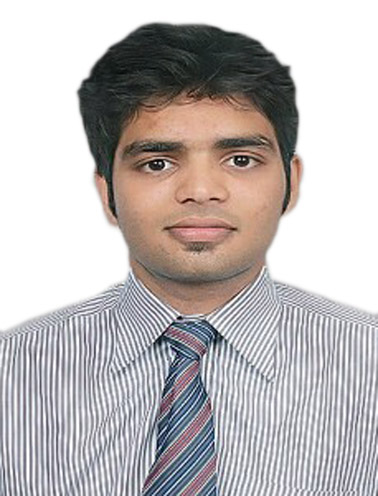
\includegraphics[width=2.5cm, height=3cm]{Photo.jpg}}}}


\newcolumntype{a}{>{\columncolor{Gray}}p}

\begin{document}
\flushleft{

\begin{longtable}{ p{13cm}a{5cm} }
%\hline
%\multicolumn{5}{|c|} \\
%\hline
\newline

{\fcolorbox{WHITE}{gray1}{\makebox[12.5cm][l]{\large{\textbf{\uppercase{Education}}}}}}\newline

\textbf{Veermata Jijabai Technological Institute (VJTI) } \newline   \textbf{CGPA} 10 \hspace{1cm}  \textbf{Percentage} - \hfill \textit{\color{gray}{\textbf{From} 14/08/2019 \textbf{To} 14/08/2023}} \newline \textbf{Core Classes}
Thermodynamics, Fluid Mechanics, Coding, Mechatronics, Entreprenuership \newline
\textbf{Professional Associations} 
\begin{itemize}[noitemsep,nolistsep]
	\item Member of Entrepreneurship-cell VJTI
    \item Member of American Society of Mechanical Engineers(ASME)(VJTI)
    \item Member of Institute of Electrical and Electronics Engineers(IEEE)(VJTI)\newline
\end{itemize} 


\textbf{South Indian Education Society(SIES)} \newline   \textbf{CGPA} -  \hspace{1cm}      \textbf{Percentage} 91\% \hfill\textit{\color{gray}{ \textbf{From} 15/06/2017 \textbf{To} 20/03/2019}}\newline \textbf{Core Classes}
Studied For JEE Mains and Advanced and various other competitive exams \newline
\textbf{Professional Associations} 
\begin{itemize}[noitemsep,nolistsep]
	\item Member of Entrepreneurship-cell VJTI
    \item Member of American Society of Mechanical Engineers(ASME)(VJTI)
    \item Member of Institute of Electrical and Electronics Engineers(IEEE)(VJTI)\newline
\end{itemize} 

\textbf{South Indian Education Society(SIES)} \newline   \textbf{CGPA} -  \hspace{1cm}      \textbf{Percentage} 91\% \hfill\textit{\color{gray}{ \textbf{From} 15/06/2017 \textbf{To} 20/03/2019}}\newline \textbf{Core Classes}
Studied For JEE Mains and Advanced and various other competitive exams \newline
\textbf{Professional Associations} 
\begin{itemize}[noitemsep,nolistsep]
	\item Member of Entrepreneurship-cell VJTI
    \item Member of American Society of Mechanical Engineers(ASME)(VJTI)
    \item Member of Institute of Electrical and Electronics Engineers(IEEE)(VJTI)\newline
\end{itemize} 


{\fcolorbox{WHITE}{gray1}{\makebox[12.5cm][l]{\large{\textbf{\uppercase{Projects}}}}}}\newline

\begin{enumerate}[noitemsep,nolistsep]
	\item {\textbf{Resume Builder}}\hfill \textit{\color{gray}{\textbf{From}: May-20 \textbf{To} July-20}}\newline
	Piranhas rarely feed on large animals; they eat smaller fish and aquatic plants. When confronted with humans, piranhas' first instinct is to flee, not attack. 
	\item {\textbf{Fan Controlled using Bluetooth}}\hfill \textit{\color{gray}{\textbf{From}: Dec-19 \textbf{To} Mar-20}}\newline
	Although most people consider piranhas to be quite dangerous, they are, for the most part, entirely harmless. Piranhas rarely feed on large animals;
	\item{\textbf{Fan Controlled using Bluetooth}}\hfill  \textit{\color{gray}{\textbf{From}: Dec-19 \textbf{To} Mar-20}}\newline
	Although most people consider piranhas to be quite dangerous, they are, for the most part, entirely harmless. Piranhas rarely feed on large animals; \newline
\end{enumerate}


{\fcolorbox{WHITE}{gray1}{\makebox[12.5cm][l]{\large{\textbf{\uppercase{Internships}}}}}}\newline

\begin{enumerate}[noitemsep,nolistsep]
	\item {\textbf{Internship at Google}}\hfill \textit{\color{gray}{\textbf{From}: Mar-20 \textbf{To} May-20}}\newline
	Developing writers can often benefit from examining an essay, a paragraph, or even a sentence to determine what makes it effective.
	\item {\textbf{Internship at Lockheed Martin}}\hfill \textit{\color{gray}{\textbf{From}: May-20 \textbf{To} Nov-20}}\newline
	 Scientists' research has revealed that viruses are by far the most abundant life forms on Earth. 
	 \item {\textbf{Internship at Lockheed Martin}}\hfill \textit{\color{gray}{\textbf{From}: May-20 \textbf{To} Nov-20}}\newline
	 Scientists' research has revealed that viruses are by far the most abundant life forms on Earth.
	 
\end{enumerate}

&
\newline
{\fcolorbox{WHITE}{gray1}{\makebox[4.5cm][l]{\textbf{\uppercase{Objective}}}}}
\flushleft{
The decision about what to put into your paragraphs begins with the germination of a seed of ideas; this "germination process" is better known as brainstorming. There are many techniques for brainstorming; whichever one you choose, this stage of paragraph development cannot be skipped.}\newline

{\fcolorbox{WHITE}{gray1}{\makebox[4.5cm][l]{\textbf{\uppercase{skills}}}}}\newline

\begin{itemize}[noitemsep,nolistsep]
	\item AutoCAD, Solidworks, AutoCAD Mechanical, Autodesk Inventor
	\item Excel, C++, HTML, Javascript, Python
	\item Management, Leadership, Organization, Public Speaking, Problem-solving, Teamwork\newline
\end{itemize}


{\fcolorbox{WHITE}{gray1}{\makebox[4.5cm][l]{\textbf{\uppercase{Hobbies}}}}}\newline

\begin{itemize}[noitemsep,nolistsep]
	\item Reading Different kinds of books, Programming, listening to classical Indian music
	\item Blogging, Volunteering, Traveling, Art, Design, Music, Reading, Video Gaming.\newline
\end{itemize}



{\fcolorbox{WHITE}{gray1}{\makebox[4.5cm][l]{\textbf{\uppercase{Achievements}}}}}\newline

\begin{itemize}[noitemsep,nolistsep]
	\item Was a part of State level football team
	\item Won many national and international level olympiads
	\item having a soft corner towards art\newline
\end{itemize}


%\hline
\end{longtable} }
\end{document}
